

What is the median of the seven data values shown?\\
A. 2\\
B. 3\\
C. 4\\
D. 9

\section*{ID: d3b9c8d8}
Group 1\\
Group 2\\
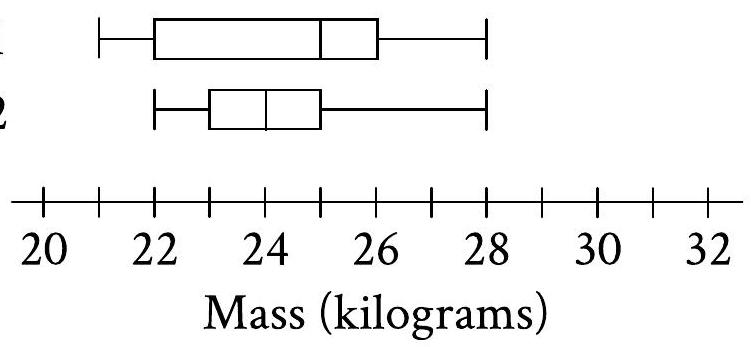
\includegraphics[max width=\textwidth, center]{2025_06_15_04f7426dc644de311e92g-02}

The box plots summarize the masses, in kilograms, of two groups of gazelles. Based on the box plots, which of the following statements must be true?\\
A. The mean mass of group 1 is greater than the mean mass of group 2.\\
B. The mean mass of group 1 is less than the mean mass of group 2 .\\
C. The median mass of group 1 is greater than the median mass of group 2 .\\
D. The median mass of group 1 is less than the median mass of group 2 .

\section*{ID: 4c774b00}
Ages of 20 Students Enrolled in a College Class

\begin{center}
\begin{tabular}{|c|c|}
\hline
Age & Frequency \\
\hline
18 & 6 \\
\hline
19 & 5 \\
\hline
20 & 4 \\
\hline
21 & 2 \\
\hline
22 & 1 \\
\hline
23 & 1 \\
\hline
30 & 1 \\
\hline
\end{tabular}
\end{center}

The table above shows the distribution of ages of the 20 students enrolled in a college class. Which of the following gives the correct order of the mean, median, and mode of the ages?\\
A. mode < median < mean\\
B. mode < mean < median\\
C. median < mode < mean\\
D. mean < mode < median\\
$4,4,4,4,8,8,8,13,13$\\
Which frequency table correctly represents the data listed?\\
A.

\begin{center}
\begin{tabular}{|c|c|}
\hline
Number & Frequency \\
\hline
4 & 4 \\
\hline
8 & 3 \\
\hline
13 & 2 \\
\hline
\end{tabular}
\end{center}

B.

\begin{center}
\begin{tabular}{|c|c|}
\hline
Number & Frequency \\
\hline
4 & 4 \\
\hline
3 & 8 \\
\hline
2 & 13 \\
\hline
\end{tabular}
\end{center}

c.

\begin{center}
\begin{tabular}{|c|c|}
\hline
Number & Frequency \\
\hline
4 & 16 \\
\hline
8 & 24 \\
\hline
13 & 26 \\
\hline
\end{tabular}
\end{center}

D.

\begin{center}
\begin{tabular}{|c|c|}
\hline
Number & Frequency \\
\hline
16 & 4 \\
\hline
24 & 8 \\
\hline
26 & 13 \\
\hline
\end{tabular}
\end{center}

\section*{ID: a456cfd2}
\begin{center}
\begin{tabular}{|c|c|}
\hline
Data value & Frequency \\
\hline
6 & 3 \\
\hline
7 & 3 \\
\hline
8 & 8 \\
\hline
9 & 8 \\
\hline
10 & 9 \\
\hline
11 & 11 \\
\hline
12 & 9 \\
\hline
13 & 0 \\
\hline
14 & 6 \\
\hline
\end{tabular}
\end{center}

The frequency table summarizes the 57 data values in a data set. What is the maximum data value in the data set?

Data set $A$ and data set $B$ each contain 5 numbers. If the mean of data set $A$ is equal to the mean of data set $B$, what is the value of $x$ ?\\
A. 77\\
B. 85\\
C. 86\\
D. 95

For a school fund-raiser, 10 students sold a total of 90 boxes of cookies. Which of the following can be calculated from this information?\\
A. The average number of boxes sold per student\\
B. The median number of boxes sold per student\\
C. The greatest number of boxes sold by one student\\
D. The least number of boxes sold by one student

\section*{ID: 3f2ee20a}
The results of two independent surveys are shown in the table below.

\begin{center}
\begin{tabular}{|c|c|c|c|}
\multicolumn{3}{c}{Men's Height} &  \\
\hline
Group & Sample size & Mean (centimeters) & Standard deviation (centimeters) \\
\hline
A & 2,500 & 186 & 12.5 \\
\hline
B & 2,500 & 186 & 19.1 \\
\hline
\end{tabular}
\end{center}

Which statement is true based on the table?\\
A. The Group A data set was identical to the Group B data set.\\
B. Group B contained the tallest participant.\\
C. The heights of the men in Group B had a larger spread than the heights of the men in Group A.\\
D. The median height of Group B is larger than the median height of Group A.

\section*{ID: d0efc1dd}
$15,14,18,17, x$\\
The mean and the median of the five numbers above are equal. Which of the following is NOT a possible value of $x$ ?\\
A. 6\\
B. 11\\
C. 16\\
D. 21

\section*{ID: 190be2fc}
Data set A consists of 10 positive integers less than 60 . The list shown gives 9 of the integers from data set A.

$$
43,45,44,43,38,39,40,46,40
$$

The mean of these 9 integers is 42 . If the mean of data set A is an integer that is greater than 42 , what is the value of the largest integer from data set A?






















































\section*{ID: 7b65bb28}
\begin{center}
\begin{tabular}{|c|c|c|c|c|}
\hline
Station 1 & Station 2 & Station 3 & Station 4 & Station 5 \\
\hline
$\$ 3.699$ & $\$ 3.609$ & $\$ 3.729$ & $\$ 3.679$ & $\$ 3.729$ \\
\hline
\end{tabular}
\end{center}

In the table above, Melissa recorded the price of one gallon of regular gas from five different local gas stations on the same day. What is the median of the gas prices Melissa recorded?\\
A. $\$ 3.679$\\
B. $\$ 3.689$\\
C. $\$ 3.699$\\
D. $\$ 3.729$

\section*{ID: be00d896}
For which of the following data sets is the mean greater than the median?\\
A. $5,5,5,5,5,5,5,5,5$\\
B. $0,10,20,30,40,50,60,70,80$\\
C. $2,4,8,16,32,64,128,256,512$\\
D. 7, 107, 107, 207, 207, 207, 307, 307, 307

The table shows the frequency of values in a data set.

\begin{center}
\begin{tabular}{|c|c|}
\hline
Value & Frequency \\
\hline
19 & 7 \\
\hline
21 & 1 \\
\hline
23 & 7 \\
\hline
25 & 4 \\
\hline
\end{tabular}
\end{center}

What is the minimum value of the data set?\\
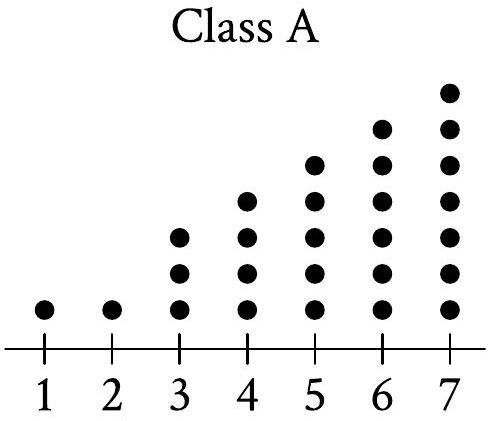
\includegraphics[max width=\textwidth, center]{2025_06_15_04f7426dc644de311e92g-24(1)}

Class B\\
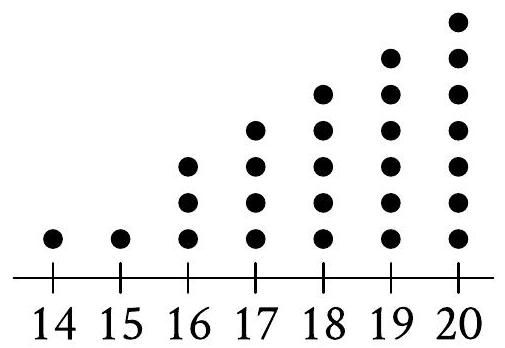
\includegraphics[max width=\textwidth, center]{2025_06_15_04f7426dc644de311e92g-24}

Each of the dot plots shown represents the number of glue sticks brought in by each student for two classes, class A and class B. Which statement best compares the standard deviations of the numbers of glue sticks brought in by each student for these two classes?\\
A. The standard deviation of the number of glue sticks brought in by each student for class $A$ is less than the standard deviation of the number of glue sticks brought in by each student for class B.\\
B. The standard deviation of the number of glue sticks brought in by each student for class $A$ is equal to the standard deviation of the number of glue sticks brought in by each student for class B.\\
C. The standard deviation of the number of glue sticks brought in by each student for class $A$ is greater than the standard deviation of the number of glue sticks brought in by each student for class B.\\
D. There is not enough information to compare these standard deviations.

A list of 10 data values is shown. $6,8,16,4,17,26,8,5,5,5$\\
What is the mean of these data?

\section*{ID: bfa8a85c}
$6,6,8,8,8,10,21$\\
Which of the following lists represents a data set that has the same median as the data set shown?\\
A. $4,6,6,6,8,8$\\
B. $6,6,8,8,10,10$\\
C. $6,8,10,10,10,12$\\
D. $8,8,10,10,21,21$

\section*{ID: fa7a0164}
The table below shows the high and low temperatures in Houston, Texas, during a five-day period.\\
Temperatures in Houston, Texas\\
(degrees Fahrenheit)

\begin{center}
\begin{tabular}{|c|c|c|c|c|c|}
\cline { 2 - 6 }
\multicolumn{1}{c|}{} & Monday & Tuesday & Wednesday & Thursday & Friday \\
\hline
High temperature & 73 & 56 & 62 & 75 & 81 \\
\hline
Low temperature & 49 & 37 & 41 & 54 & 63 \\
\hline
\end{tabular}
\end{center}

What was the mean low temperature, in degrees Fahrenheit, during the five-day period?\\
A. 48.8\\
B. 49\\
C. 59\\
D. 59.1

\section*{ID: 708590d7}
Data set A: 1, 2, 3, 4, 5, 6, 7\\
Data set B: 1, 1, 2, 2, 3, 3, 4

Which of the following statements correctly compares the means of data set A and data set B?\\
A. The mean of each data set is 2 .\\
B. The mean of each data set is 4 .\\
C. The mean of data set $A$ is less than the mean of data set $B$.\\
D. The mean of data set $A$ is greater than the mean of data set $B$.

Each of the following frequency tables represents a data set. Which data set has the greatest mean?\\
A.

\begin{center}
\begin{tabular}{|c|c|}
\hline
Value & Frequency \\
\hline
70 & 4 \\
\hline
80 & 5 \\
\hline
90 & 6 \\
\hline
100 & 7 \\
\hline
\end{tabular}
\end{center}

B.

\begin{center}
\begin{tabular}{|c|c|}
\hline
Value & Frequency \\
\hline
70 & 6 \\
\hline
80 & 6 \\
\hline
90 & 6 \\
\hline
100 & 6 \\
\hline
\end{tabular}
\end{center}

C.

\begin{center}
\begin{tabular}{|c|c|}
\hline
Value & Frequency \\
\hline
70 & 7 \\
\hline
80 & 6 \\
\hline
90 & 6 \\
\hline
100 & 7 \\
\hline
\end{tabular}
\end{center}

D.

\begin{center}
\begin{tabular}{|c|c|}
\hline
Value & Frequency \\
\hline
70 & 8 \\
\hline
80 & 5 \\
\hline
90 & 5 \\
\hline
100 & 8 \\
\hline
\end{tabular}
\end{center}

Each value in the data set shown represents the height, in centimeters, of a plant.

$$
6,10,13,2,15,22,10,4,4,4
$$

What is the mean height, in centimeters, of these plants?

The number of acres of useful timberland in 13 counties in California is summarized in the box plot above. Which of the following is closest to the median number of acres?\\
A. 4,399\\
B. 7,067\\
C. 8,831\\
D. 10,595

The mean amount of time that the 20 employees of a construction company have worked for the company is 6.7 years. After one of the employees leaves the company, the mean amount of time that the remaining employees have worked for the company is reduced to 6.25 years. How many years did the employee who left the company work for the company?\\
A. 0.45\\
B. 2.30\\
C. 9.00\\
D. 15.25























\section*{ID: c54b92a2}
A study was conducted on the production rates for a company that produces tractor wheels. The table below shows the number of wheels made during 11 consecutive one-hour production periods.

\begin{center}
\begin{tabular}{|c|c|}
\hline
\begin{tabular}{c}
One- \\
hour \\
period \\
\end{tabular} & \begin{tabular}{c}
Number \\
of \\
wheels \\
made \\
\end{tabular} \\
\hline
A & 24 \\
\hline
B & 24 \\
\hline
C & 21 \\
\hline
D & 21 \\
\hline
E & 21 \\
\hline
F & 19 \\
\hline
G & 24 \\
\hline
H & 24 \\
\hline
I & 19 \\
\hline
J & 22 \\
\hline
K & 23 \\
\hline
\end{tabular}
\end{center}

What is the range of the number of wheels made for the 11 one-hour periods?\\
A. 5.5\\
B. 5.0\\
C. 4.5\\
D. 4.0

\section*{ID: 5c3c2e3c}
The weights, in pounds, for 15 horses in a stable were reported, and the mean, median, range, and standard deviation for the data were found. The horse with the lowest reported weight was found to actually weigh 10 pounds less than its reported weight. What value remains unchanged if the four values are reported using the corrected weight?\\
A. Mean\\
B. Median\\
C. Range\\
D. Standard deviation\\
$71,72,73,76,77,79,83,87,93$\\
What is the median of the data shown?\\
A. 71\\
B. 77\\
C. 78\\
D. 79

\section*{ID: 9110c120}
Data set A: $5,5,5,5,5,5,5,5,5$\\
Data set B: 5, 5, 5, 5, 5, 5, 5, 5, 5, 100

Which of the following statements about the means and medians of data set $A$ and data set $B$ is true?\\
A. Only the means are different.\\
B. Only the medians are different.\\
C. Both the means and the medians are different.\\
D. Neither the means nor the medians are different.

\section*{ID: d1db8def}
\begin{center}
\begin{tabular}{|l|l|}
\hline
Response & Frequency \\
\hline
Once a week or more & 3 \\
\hline
Two or three times a month & 16 \\
\hline
About once a month & 26 \\
\hline
A few times a year & 73 \\
\hline
Almost never & 53 \\
\hline
Never & 29 \\
\hline
Total & 200 \\
\hline
\end{tabular}
\end{center}

The table gives the results of a survey of 200 people who were asked how often they see a movie in a theater. How many people responded either "never" or "almost never"?\\
A. 24\\
B. 53\\
C. 82\\
D. 118

\section*{Data Set A}
\begin{center}
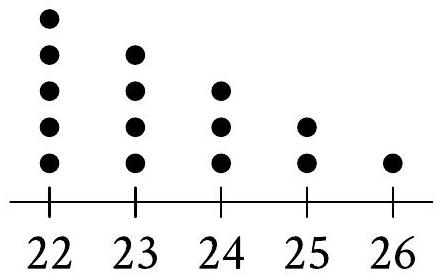
\includegraphics[max width=\textwidth]{2025_06_15_04f7426dc644de311e92g-38}
\end{center}

The dot plot represents the 15 values in data set $A$. Data set $B$ is created by adding 56 to each of the values in data set $A$. Which of the following correctly compares the medians and the ranges of data sets $A$ and $B$ ?\\
A. The median of data set $B$ is equal to the median of data set $A$, and the range of data set $B$ is equal to the range of data set A.\\
B. The median of data set $B$ is equal to the median of data set $A$, and the range of data set $B$ is greater than the range of data set A.\\
C. The median of data set $B$ is greater than the median of data set $A$, and the range of data set $B$ is equal to the range of data set A.\\
D. The median of data set $B$ is greater than the median of data set $A$, and the range of data set $B$ is greater than the range of data set A.

\section*{ID: 55cfaf22}
Data set X: 5, 9, 9, 13\\
Data set Y: 5, 9, 9, 13, 27\\
The lists give the values in data sets $X$ and $Y$. Which statement correctly compares the mean of data set $X$ and the mean of data set $Y$ ?\\
A. The mean of data set $X$ is greater than the mean of data set $Y$.\\
B. The mean of data set $X$ is less than the mean of data set $Y$.\\
C. The means of data set $X$ and data set $Y$ are equal.\\
D. There is not enough information to compare the means.

\section*{ID: 820d7a73}
\begin{center}
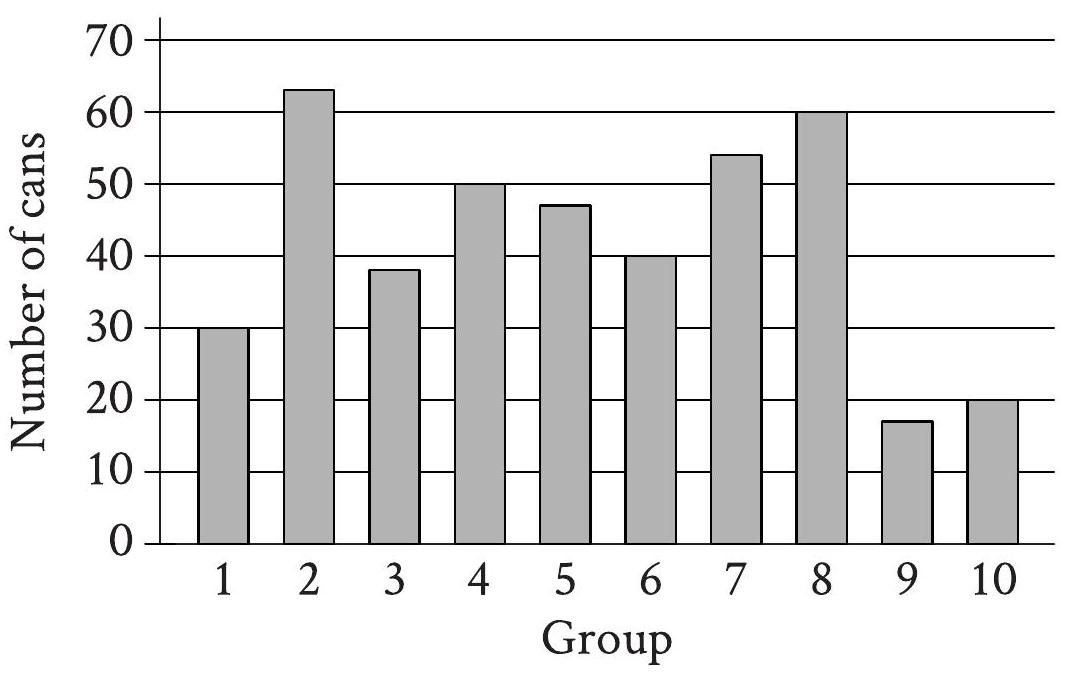
\includegraphics[max width=\textwidth]{2025_06_15_04f7426dc644de311e92g-40}
\end{center}

The bar graph shows the distribution of 419 cans collected by 10 different groups for a food drive. How many cans were collected by group 6?

If $a$ is the mean and $b$ is the median of nine consecutive integers, what is the value of $|a-b|$ ?

ID: 4bb25495\\
Five Smallest Countries in 2016

\begin{center}
\begin{tabular}{|c|c|}
\hline
Country & \begin{tabular}{c}
Land area \\
(square kilometers) \\
\end{tabular} \\
\hline
Monaco & 2.0 \\
\hline
Nauru & 21 \\
\hline
San Marino & 61 \\
\hline
Tuvalu & 26 \\
\hline
Vatican City & 0.44 \\
\hline
\end{tabular}
\end{center}

The table above shows the land area, in square kilometers, of the five smallest countries of the world in 2016. Based on the table, what is the mean land area of the 5 smallest countries in 2016, to the nearest square kilometer?\\
A. 20\\
B. 22\\
C. 61\\
D. 110

Data set A consists of the heights of 75 objects and has a mean of 25 meters. Data set B consists of the heights of 50 objects and has a mean of 65 meters. Data set $C$ consists of the heights of the 125 objects from data sets $A$ and $B$. What is the mean, in meters, of data set C?

Data set $F$ consists of 55 integers between 170 and 290 . Data set $G$ consists of all the integers in data set $F$ as well as the integer 10 . Which of the following must be less for data set $F$ than for data set $G$ ?\\
I. The mean\\
II. The median\\
A. I only\\
B. II only\\
C. I and II\\
D. Neither I nor II\\
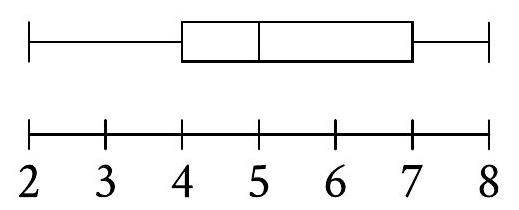
\includegraphics[max width=\textwidth, center]{2025_06_15_04f7426dc644de311e92g-45}

The box plot summarizes 15 data values. What is the median of this data set?\\
A. 2\\
B. 3\\
C. 5\\
D. 8

\section*{ID: 2a59eb45}
Data set A consists of the heights of 75 buildings and has a mean of 32 meters. Data set B consists of the heights of 50 buildings and has a mean of 62 meters. Data set $C$ consists of the heights of the 125 buildings from data sets $A$ and $B$. What is the mean, in meters, of data set C?\\
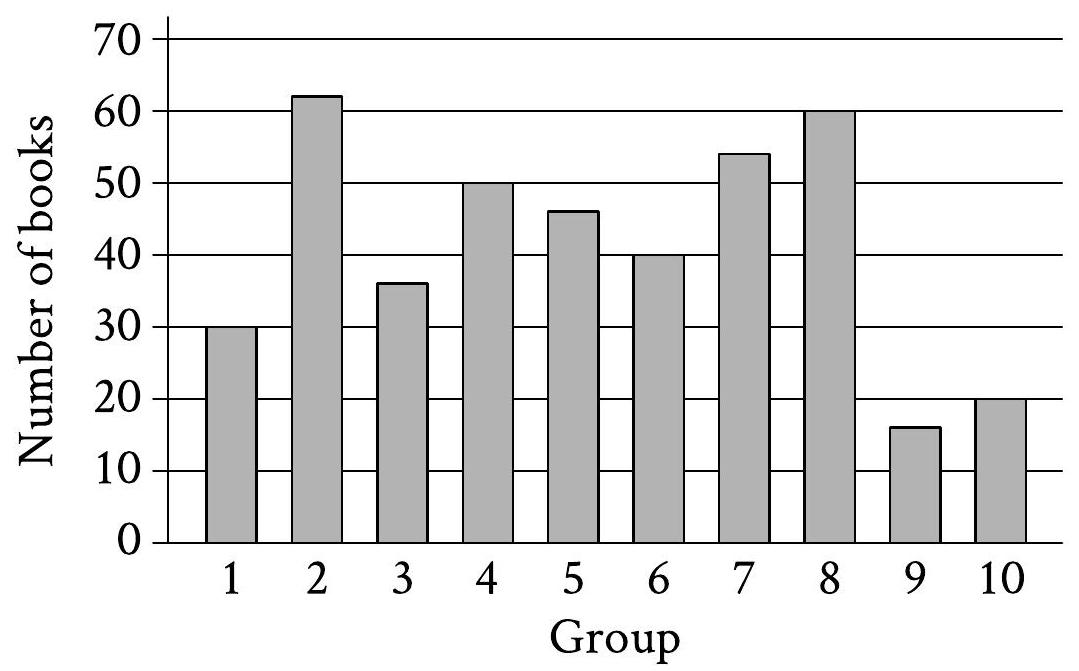
\includegraphics[max width=\textwidth, center]{2025_06_15_04f7426dc644de311e92g-47}

The bar graph shows the distribution of 414 books collected by 10 different groups for a book drive. How many books were collected by group 1?\\
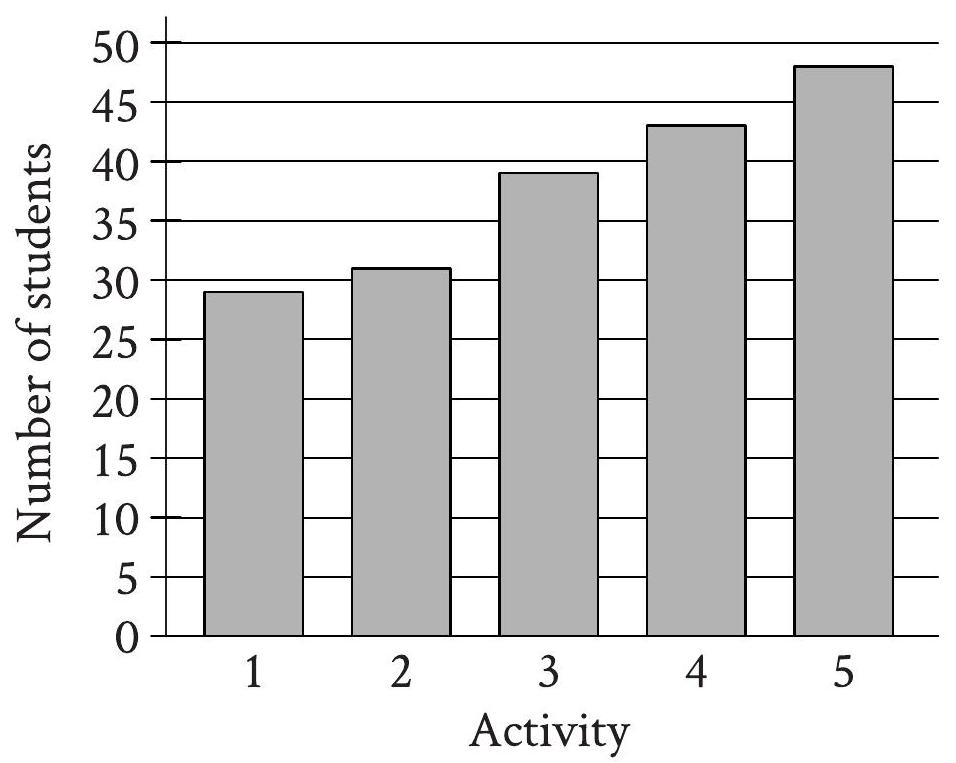
\includegraphics[max width=\textwidth, center]{2025_06_15_04f7426dc644de311e92g-48}

A group of students voted on five after-school activities. The bar graph shows the number of students who voted for each of the five activities. How many students chose activity 3 ?\\
A. 25\\
B. 39\\
C. 48\\
D. 50

\section*{ID: 9d935bd8}
Percent of Residents Who Earned a Bachelor's Degree or Higher

\begin{center}
\begin{tabular}{|c|c|}
\hline
State & Percent of residents \\
\hline
State A & $21.9 \%$ \\
\hline
State B & $27.9 \%$ \\
\hline
State C & $25.9 \%$ \\
\hline
State D & $19.5 \%$ \\
\hline
State E & $30.1 \%$ \\
\hline
State F & $36.4 \%$ \\
\hline
State G & $35.5 \%$ \\
\hline
\end{tabular}
\end{center}

A survey was given to residents of all 50 states asking if they had earned a bachelor's degree or higher. The results from 7 of the states are given in the table above. The median percent of residents who earned a bachelor's degree or higher for all 50 states was $26.95 \%$. What is the difference between the median percent of residents who earned a bachelor's degree or higher for these 7 states and the median for all 50 states?\\
A. $0.05 \%$\\
B. $0.95 \%$\\
C. $1.22 \%$\\
D. $7.45 \%$

\section*{ID: 9e2bf782}
A fish hatchery has three tanks for holding fish before they are introduced into the wild. Ten fish weighing less than 5 ounces are placed in tank A. Eleven fish weighing at least 5 ounces but no more than 13 ounces are placed in tank B. Twelve fish weighing more than 13 ounces are placed in tank C. Which of the following could be the median of the weights, in ounces, of these 33 fish?\\
A. 4.5\\
B. 8\\
C. 13.5\\
D. 15

\section*{ID: a9647302}
\begin{center}
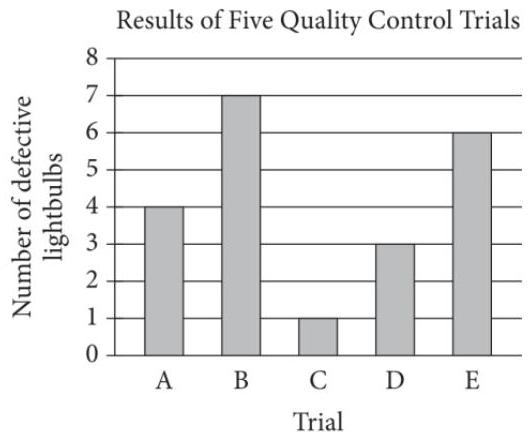
\includegraphics[max width=\textwidth]{2025_06_15_04f7426dc644de311e92g-51}
\end{center}

For quality control, a company that manufactures lightbulbs conducted five different trials. In each trial, 500 different lightbulbs were tested. The bar graph above shows the number of defective lightbulbs found in each trial. What is the mean number of defective lightbulbs for the five trials?\\
A. 4.0\\
B. 4.2\\
C. 4.6\\
D. 5.0

2, 10, 3, 7, 6

The mean of the list of numbers above is what fraction of the sum of the five numbers?

\begin{center}
\begin{tabular}{|c|c|c|c|c|c|c|}
\hline
 & \multicolumn{6}{|c|}{Masses (kilograms)} \\
\hline
Andrew & 2.4 & 2.5 & 3.6 & 3.1 & 2.5 & 2.7 \\
\hline
Maria & $x$ & 3.1 & 2.7 & 2.9 & 3.3 & 2.8 \\
\hline
\end{tabular}
\end{center}

Andrew and Maria each collected six rocks, and the masses of the rocks are shown in the table above. The mean of the masses of the rocks Maria collected is 0.1 kilogram greater than the mean of the masses of the rocks Andrew collected. What is the value of $x$ ?

\section*{ID: 869a32f1}
The high temperature, in degrees Fahrenheit ( ${ }^{\circ} \mathrm{F}$ ), in a certain city was recorded for each of 5 days. The data are shown below.

\begin{center}
\begin{tabular}{|c|c|c|c|c|c|}
\hline
Day & 1 & 2 & 3 & 4 & 5 \\
\hline
High temperature ( ${ }^{\circ}$ F) & 81 & 80 & 81 & 81 & 82 \\
\hline
\end{tabular}
\end{center}

Over this 5-day period, which of the following is NOT equal to $81^{\circ} \mathrm{F}$ ?\\
A. Median of the high temperatures\\
B. Mean of the high temperatures\\
C. Mode of the high temperatures\\
D. Range of the high temperatures

\section*{ID: 6670e407}
Number of High School Students Who\\
Completed Summer Internships

\begin{center}
\begin{tabular}{|l|c|c|c|c|c|}
\hline
\multirow{2}{*}{\begin{tabular}{l}
High \\
school \\
\end{tabular}} & \multicolumn{5}{|c|}{Year} \\
\cline { 2 - 6 }
 & $\mathbf{2 0 0 8}$ & $\mathbf{2 0 0 9}$ & $\mathbf{2 0 1 0}$ & $\mathbf{2 0 1 1}$ & $\mathbf{2 0 1 2}$ \\
\hline
Foothill & 87 & 80 & 75 & 76 & 70 \\
\hline
Valley & 44 & 54 & 65 & 76 & 82 \\
\hline
Total & 131 & 134 & 140 & 152 & 152 \\
\hline
\end{tabular}
\end{center}

The table above shows the number of students from two different high schools who completed summer internships in each of five years. No student attended both schools. Which of the following statements are true about the number of students who completed summer internships for the 5 years shown?

\begin{enumerate}
  \item The mean number from Foothill High School is greater than the mean number from Valley High School.
  \item The median number from Foothill High School is greater than the median number from Valley High School.\\
A. I only\\
B. II only\\
C. I and II\\
D. Neither I nor II
\end{enumerate}

For a certain computer game, individuals receive an integer score that ranges from 2 through 10. The table below shows the frequency distribution of the scores of the 9 players in group $A$ and the 11 players in group $B$.

\begin{center}
\begin{tabular}{|l|l|l|}
\hline
\multirow{2}{*}{Score} & \multicolumn{2}{|c|}{Score Frequencies} \\
\hline
 & Group A & Group B \\
\hline
2 & 1 & 0 \\
\hline
3 & 1 & 0 \\
\hline
4 & 2 & 0 \\
\hline
5 & 1 & 4 \\
\hline
6 & 3 & 2 \\
\hline
7 & 0 & 0 \\
\hline
8 & 0 & 2 \\
\hline
9 & 1 & 1 \\
\hline
10 & 0 & 2 \\
\hline
Total & 9 & 11 \\
\hline
\end{tabular}
\end{center}

The median of the scores for group $B$ is how much greater than the median of the scores for group A?


